\documentclass[11pt]{scrartcl}
\usepackage[sexy]{evan}
\usepackage{graphicx}

\newcommand{\N}{\mathbb{N}}
\newcommand{\Z}{\mathbb{Z}}
\newcommand{\F}{\mathbb{F}}
\newcommand{\Q}{\mathbb{Q}}
\newcommand{\R}{\mathbb{R}}
\newcommand{\C}{\mathbb C}


\newcommand{\Vu}{\mathbf{u}}
\newcommand{\Vv}{\mathbf{v}}
\newcommand{\Vw}{\mathbf{w}}
\newcommand{\Vx}{\mathbf{x}}
\newcommand{\Ve}{\mathbf{e}}
\newcommand{\Vc}{\mathbf{c}}
\newcommand{\Vb}{\mathbf{b}}



\newcommand{\Va}{\mathbf{a}}

\newcommand{\Vhx}{\mathbf{\hat{x}}}

\newcommand{\Vy}{\mathbf{y}}
\newcommand{\Vz}{\mathbf{z}}
\newcommand{\Vo}{\mathbf{0}}

%From Topology
\newcommand{\cT}{\mathcal{T}}
\newcommand{\cB}{\mathcal{B}}
\newcommand{\cC}{\mathcal{C}}

\usepackage{answers}
\Newassociation{hint}{hintitem}{all-hints}
\renewcommand{\solutionextension}{out}
\renewenvironment{hintitem}[1]{\item[\bfseries #1.]}{}
\declaretheorem[style=thmbluebox,name={Theorem}]{thm}

\begin{document}
\title{CS 189}
\author{Vishal Raman}
\thispagestyle{empty}
$ $
\vfill
\begin{center}

\centerline{\huge \textbf{CS 189 Lecture Notes, Fall 2020}}
\centerline{\Large \textbf{Machine Learning} } 
\centerline{Professor: Anant Sahai, Jennifer Listgarten, Jitendra Malik}
\centerline{Vishal Raman}
\end{center}
\vfill
$ $
\newpage
\thispagestyle{empty}
\tableofcontents
\newpage
%\maketitle
\section{August 31th, 2020}
\subsection{Basics}
We would like to understand patterns from data, which means being able to predict.  If a pattern exists, it will be confirmed with prediction, to some extent.

\begin{definition}[Supervised Learning] We have data $\Vx_i$, outputs $y_i$. We have a success if given $\Vx$, not in our data, we can predict $\hat{y}$ which is "correct".
\end{definition}

There are two kinds of outputs we can consider:
\begin{itemize}
\item Continuous scalars of vectors, which are real or complex valued.  We consider problems of this form "regression problems".
\item Categorical "quantities", ex. "dog" vs "cat" vs "banana".  We consider problems of this form "classification problems".  We immediately have the problem of representation for categorical variables.
\end{itemize}

The usual solution is as follows:
\begin{definition}[One-hot Encoding] We encode a categorical variable as a vector, where entries correspond to boolean variables on the categories.   In the case of binary variables, it suffices to take $y = \pm 1$, for each category.
\end{definition}
\begin{example} $\hat{y} = [1, 0, 0]$ corresponds to Dog, Not Cat, Not Banana.  
\end{example}

Question: Can all problems be reduced to regression?

Answer:  It turns out that regression-type problems can be mended as optimization problems.  For this reason, we try to cast ML as optimization problems, which will sometimes have a regression-type feeling to them.

The levels of an ML problem:
\begin{enumerate}
\item Problem: We have data(a collection of $(x_i, y_i)$ pairs) and want to predict $\hat{y}$ with $x_i$.
\item Model: what kind of pattern are we looking for?  (finding all possible patterns is impossibly difficult)
\item Approach: a learning algorithm, which is done by framing and solving an Optimization problem.
\end{enumerate}

\begin{definition}[Least-Squares Problem] Find $\Vw$ that minimizes $\|A\Vw - \Vb\|^2$.
\end{definition}

\begin{example} We would like to predict the orbit of Cerus.  Problem: We have take $(x, y)$ pairs in the plane.  
Model: Find an elliptical orbit for Cerus.  
\end{example}
We model the problem as a Least-Squares problem. We have points $(x_1, y_1), (x_2, y_2), \dots, (x_n, y_n)$.  Any conic section is of the form $w[0]x^2 + w[1]y^2 + w[2]xy + w[3]x + w[4]y + w[5] = 1$ (this is a somewhat relaxed approach to the problem, but it is easy to implement).

We find $\text{arg}\min_{\Vw} \| [x_i^2, y_i^2, x_iy_i, x_i, y_i, 1]\Vw - [\mathbf{1}]\|^2$.   We call the $x_i^2, y_i^2, x_iy_i, x_i, y_i$ features.

\subsection{Features}
\begin{definition}[Features] The components of the pattern that we are trying to learn.  It is a mapping from the input data.
\end{definition}
Picking the features is where ML is more an art than a science, and usually requires domain knowledge to be successful.
\begin{definition}[Linear Regression] The desired pattern, a linear combination of features.
\end{definition}
\subsection{Classification Comments}
\begin{definition}[Signature Approach] Every class $\ell$ is associated to a signature $\Vw_\ell$.  Given features $\Vx$, we compute $\text{arg}\max_{\ell} \Vx^T \Vw_\ell$.
\end{definition}
The learning problem is to find the $\Vw_\ell$.  For the binary case, with two signatures, we wish to check $\Vx^T \Vw_1 > \Vx^T\Vw_2\Rightarrow \Vx^T(\Vw_1 - \Vw_2) > 0$, so it reduces to a single signature.

We can learn the $\Vw_\ell$ using one-hot-encoding to set $\Vy$.  
%include graphics
\begin{center}
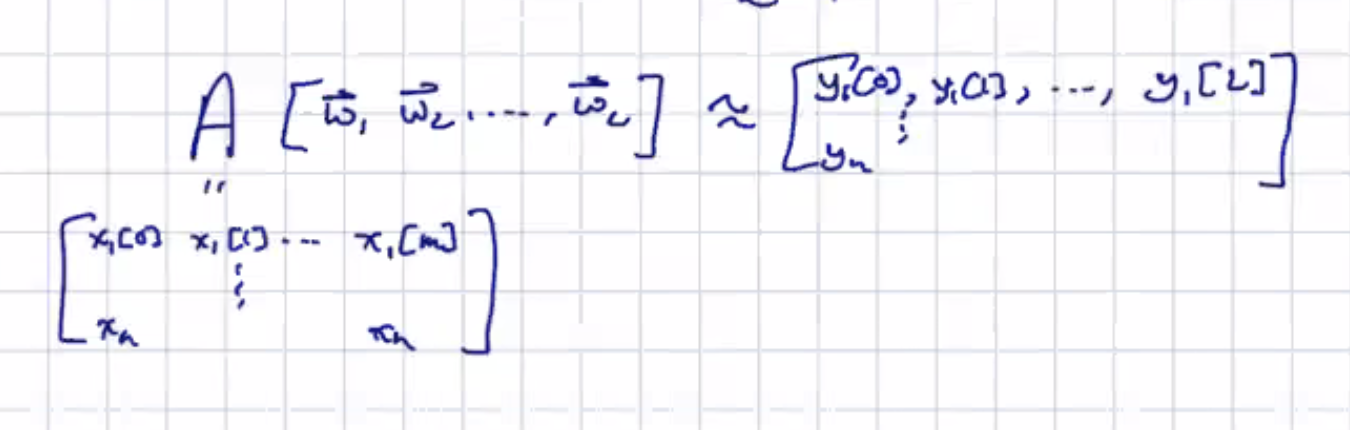
\includegraphics[scale = 0.5]{matrixMultiply.png}
\end{center}
It suffices to take $\hat{w} = (A^TA)^{-1}A^TY$.


Where do features come from?
\begin{itemize}
\item Domain-specific knowledge
\item Universal Function Approximation: any function on a compact set can be approximated to any chosen accuracy.
\end{itemize}
\subsection{Conditioning and Ridge Regularization}
What can go wrong with squared-error approaches?  The first clear problem is that $A^TA$ might not be invertible.

We take an SVD approach to $(A^TA)^{-1}A^T$: let $A = U\Sigma V^T$.
\begin{center}
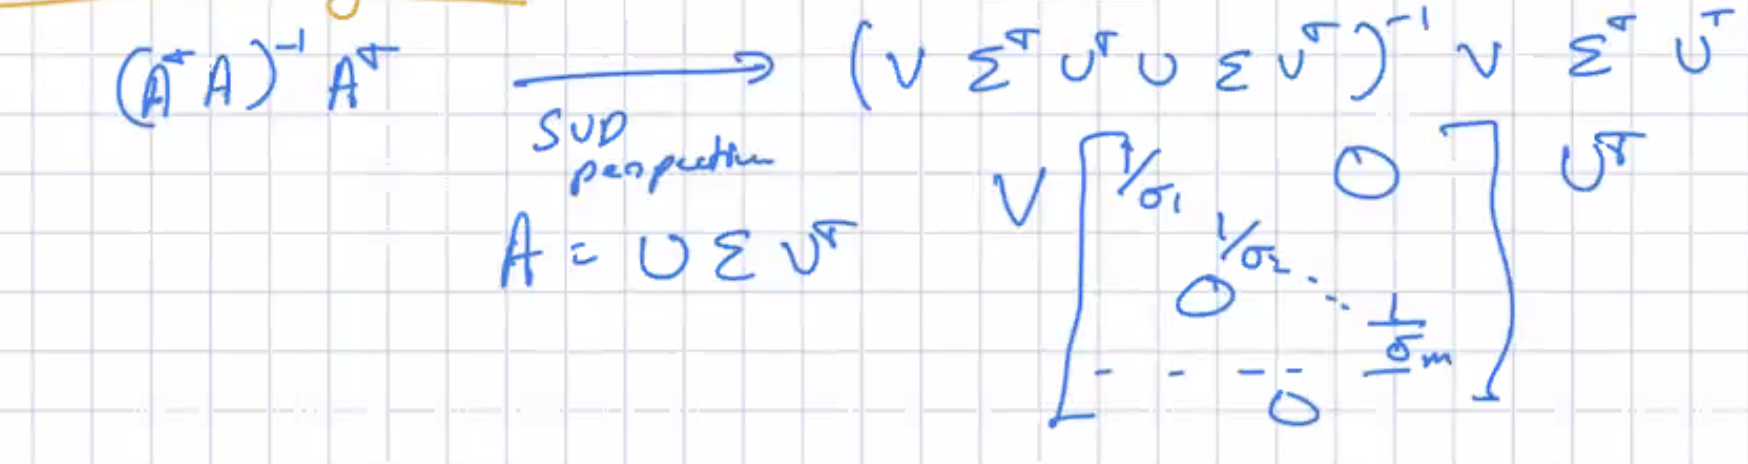
\includegraphics[scale=0.5]{svd.png}
\end{center}
Notice that we have reciprocals of singular values, which will blow up for small values.  This is a problem because the noise in the data will be amplified by very large values. 

 We could take a dimensionality reduction(PCA) approach to kill off small singular values, or we take a hack: compute $(A^TA + \lambda I)^{-1}A^T$.  We now have $\hat{w}  = (A^TA + \lambda I)^{-1}A^T Y$.  We note that 
$$\frac{1}{\sigma_j + \lambda} = \frac{1}{\sigma_j}\left (\frac{1}{1 + \frac{\lambda}{\sigma_j}}\right ),$$
which acts as a high-pass filter.  This is known as "ridge regularization".
\end{document}
